

\lstset{
 columns=fixed,       
 numbers=left,                                        % 在左侧显示行号
 numberstyle=\tiny\color{gray},                       % 设定行号格式
 frame=none,                                          % 不显示背景边框
 backgroundcolor=\color[RGB]{245,245,244},            % 设定背景颜色
 keywordstyle=\color[RGB]{40,40,255},                 % 设定关键字颜色
 numberstyle=\footnotesize\color{darkgray},           
 commentstyle=\it\color[RGB]{0,96,96},                % 设置代码注释的格式
 stringstyle=\rmfamily\slshape\color[RGB]{128,0,0},   % 设置字符串格式
 showstringspaces=false,                              % 不显示字符串中的空格
 language=c,                                        % 设置语言
}


\chapter{固定控制类NBIOT应用的设计与实现}
基于NB-IOT的终端应用大致分为4类,分别是固定上报类,固定控制类,移动上报类和移动控制类。不同类别的应用因为数据的实时性、数据量、部署环境等的不同,对网络以及电源的需求也不同。例如对于固定控制类,
由于设备部署位置固定,常有外部电源支持,需要较强的实时性,所以对功耗需求不高,需要模块时刻保持在线状态。接下来将以BC35G模块为基础,结合stm32开发板,实现一个固定控制类物联网终端实例,演示BC35G
模块通过开发板控制通信操作,物联网应用开发以及CoAP通信过程。

\section{总体设计}

\subsection{设计目标}
使用stm32开发板,BC35G模块以及华为物联网平台,设计一个物联网演示应用。通过CoAP接入华为云平台协议接入华为云平台,能够通过华为云平台给开发板下发开灯、关灯,响铃操作,并且开发板定时上报自身LED
和无源蜂鸣器状态给华为云平台。

\subsection{设计任务}

对于一个物联网应用,其基本架构应如图\ref{物联网应用总体架构}。主要由终端设备、物联网平台和业务应用组成。终端设备作为物联网的感知层,是整个应用的核心资源,物联网平台用于管理终端设备的注册、固件
更新等,同时屏蔽复杂的设备接口,处理业务应用与终端设备的通信。业务应用则通过物联网平台暴露出的restful接口,面向用户以及管理员,为用户提供最终的服务和管理员对终端设备的管理。

\begin{figure}[h]
    \centering
  	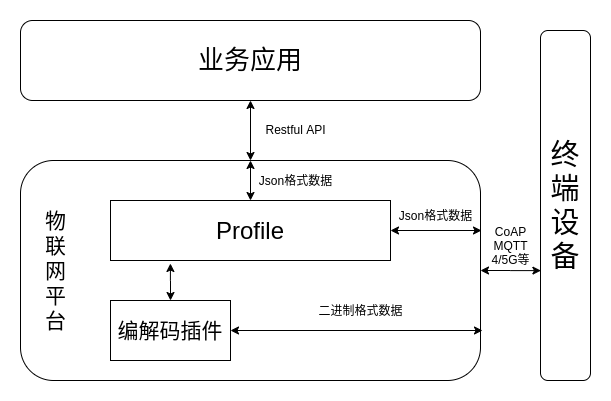
\includegraphics[width=10cm]{物联网应用总体架构.png}
	\caption{物联网应用总体架构}
	\label{物联网应用总体架构}
\end{figure}

本次设计任务中,终端设备将通过CoAP协议与华为云平台进行二进制数据交互,并由华为云平台暴露出restful接口,所以主要工作集中与华为云平台和终端设备的开发。对于华为云平台,
需要定义设备的profile文件,以标识设备特征以及能力,也需要开发编解码插件,用于json和二进制数据的转换;对于终端设备,同样首先需要实现与华为物联网平台一致的编解码插件逻辑,从而能与物联网平台交互,
然后需要开发控制stm32资源的能力,从而使开发板能
根据华为物联网平台的相应指令做出对应动作。

\subsection{详细设计}

BC35G模块将通过一组串口与stm32开发板通信,需要使用stm32开发板上的一组串口,作为接受华为云平台控制消息和stm32开发板上传自身资源状态的通告,所以BC35G模块与stm32开发板需以图\ref{硬件连接}的方式连接。
\begin{figure}[h]
    \centering
  	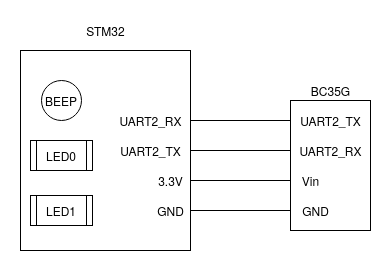
\includegraphics[width=9cm]{硬件连接.png}
	\caption{硬件连接}
	\label{硬件连接}
\end{figure}

如图\ref{硬件连接}所示,stm32开发板上主要使用的控制资源是一对发光二级管和一个无源蜂鸣器,所以华为物联网平台与设备终端之间交互的消息应该有三类,分别用于终端设备上报资源状态(resource\_info),
物联网平台下发的资源控制命令(set\_resource)和物联网平台下发的资源查询命令(query\_resource)。

resource\_info需要包含3个系统资源的状态,定义为led0,led1和beep,使用0/1代表关闭、开启状态,所以使用uint8编码;
set\_resouce用于设置资源状态,所以使用num代表资源编号,分别对用 led0(0),led1(1),beep(2),state代表需要将资源设置成的状态;
query\_resouce类似set\_resource,使用num代表需要查询状态的资源编号;
三类消息中的messageId用于编解码插件识别消息类型并进行处理。
详细的消息定义如表\ref{消息模板}:

\begin{table}[h]
\caption{消息模板}
\begin{tabular}{|c|c|c|c|c|c|}
\toprule
消息类型 & 字段名称 & 数据类型 & 偏移量 & 字段解释 & 消息解释 \\
\hline
\multirow{4}{*}{resource\_info} & messageId & uint8 & 0-1 & 消息类型编号:2 & \multirow{4}{*}{模块上报消息} \\
\cmidrule{2-5}
& led0 & uint8 & 1-2 & led0 状态 & \\
\cmidrule{2-5}
& led1 & uint8 & 2-3 & led1 状态 & \\
\cmidrule{2-5}
& beep & uint8 & 3-4 & beep 状态 & \\
\hline
\multirow{3}{*}{set\_resource} & messageId & uint8 & 0-1 & 消息类型编号:0 & \multirow{3}{*}{模块控制消息} \\
\cmidrule{2-5}
& num & uint8 & 1-2 & 需要控制的资源编号 & \\
\cmidrule{2-5}
& state & uint8 & 2-3 & 资源状态 & \\
\hline
\multirow{3}{*}{query\_resource} & messageId & uint8 & 0-1 & 消息类型编号:1 & \multirow{3}{*}{触发模块上报} \\
\cmidrule{2-5}
& num & uint8 & 1-2 & 需要上报的资源编号 & \\
\bottomrule
\end{tabular}
\label{消息模板}
\end{table}

\section{华为云平台应用开发}
华为 OceanConnect物联网平台作为一个连接业务应用和物联网设备的中间层,提供了海量设备接入管理,屏蔽复杂的设备接口,支持多网络、多协议
的终端设备接入,配合华为云其他产品同时使用,可以快速构筑物联网应用。
%\begin{figure}[h]
%    \floatcontinue
%	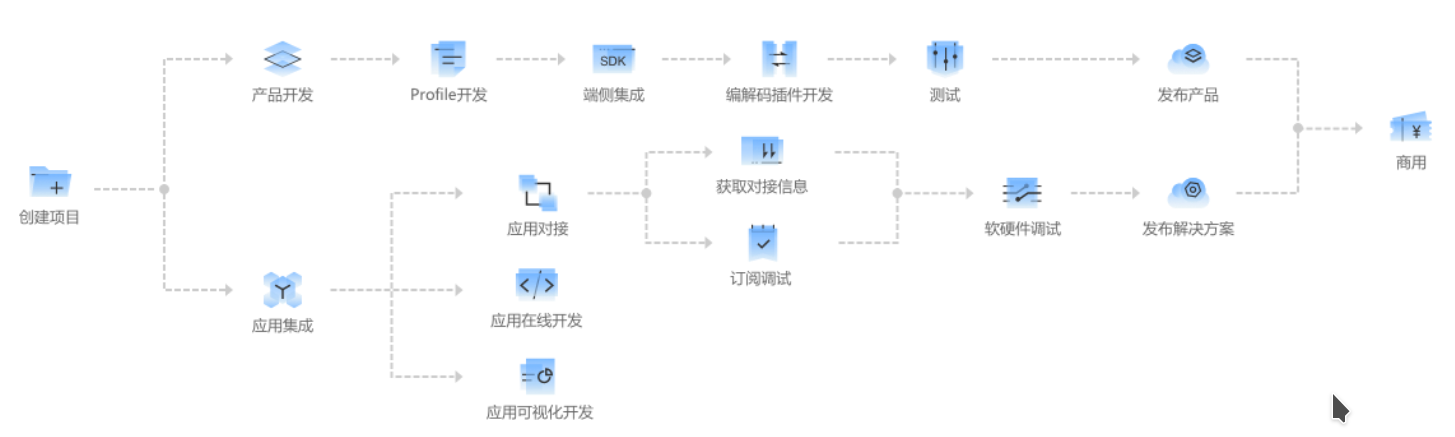
\includegraphics[width=20cm]{oc流程.png}
%	\caption{oc流程}
%	\label{oc流程}
%\end{figure}

\subsection{创建项目}
项目作为华为物联网平台上的一个应用空间,用于区分不同应用场景下的调试开发,每个项目有一个应用ID作为项目的唯一标识,华为物联网平台用于区
分通过Restful接口到来的应用服务器请求以路由到对应的项目空间。

在华为OceanConnect开发中心上创建项目如图\ref{创建项目1},获取平台分配的应用ID和应用秘钥,用于后期应用服务器连接华为物联网平台。
\begin{figure}[H]
    \centering
	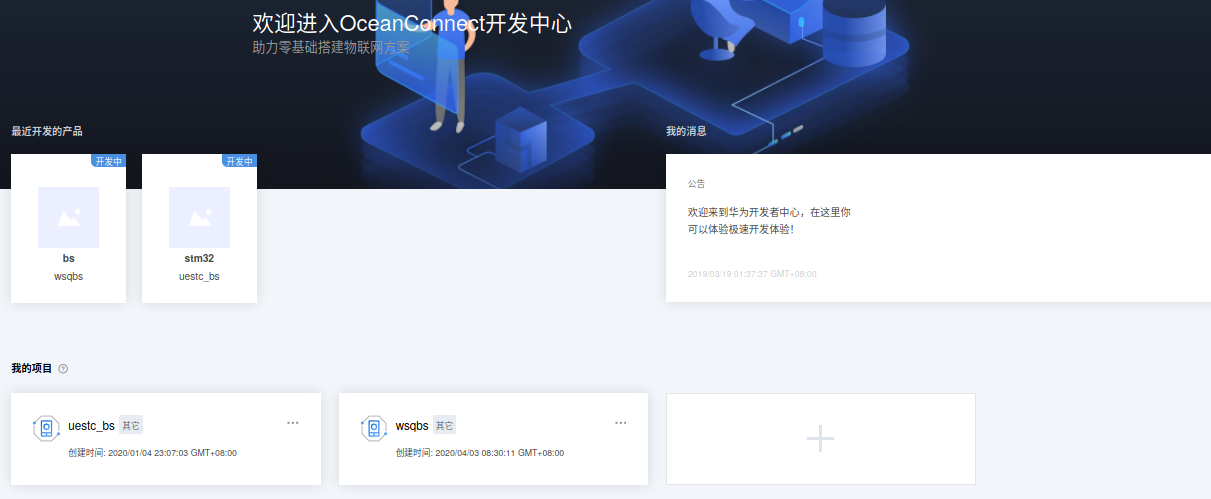
\includegraphics[width=8cm]{创建项目1.png}
	\caption{创建项目1}
	\label{创建项目1}
\end{figure}
\begin{figure}[H]
    \centering
	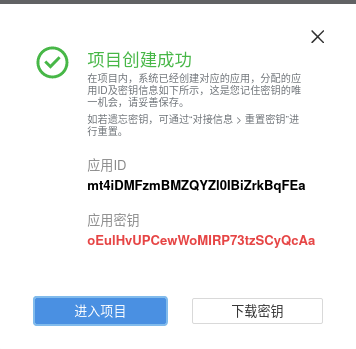
\includegraphics[width=8cm]{创建项目3.png}
	\caption{创建项目3}
	\label{创建项目3}
\end{figure}
\begin{figure}[H]
    \centering
	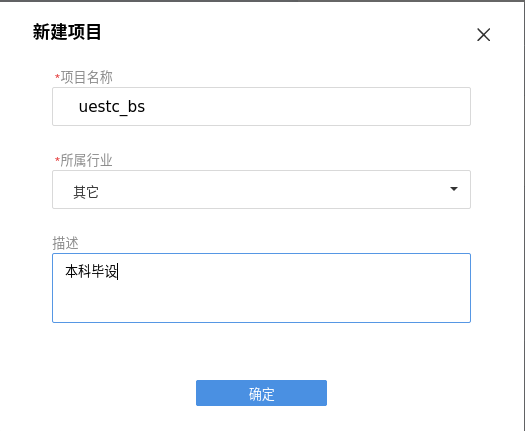
\includegraphics[width=8cm]{创建项目2.png}
	\caption{创建项目2}
	\label{创建项目2}
\end{figure}


\subsection{定义产品}
产品是指一类具备相同能力和特征的设备,一个产品包含产品模型、编解码插件等资源。应用层协议选用CoAP协议。由于使用JSON的数据格式对能耗消耗太大,
不适用于物联网设备,所以选用二进制码流的数据格式,通过开发编解码插件解析。定义产品如图\ref{oc产品定义}。
\begin{figure}[H]
    \centering
	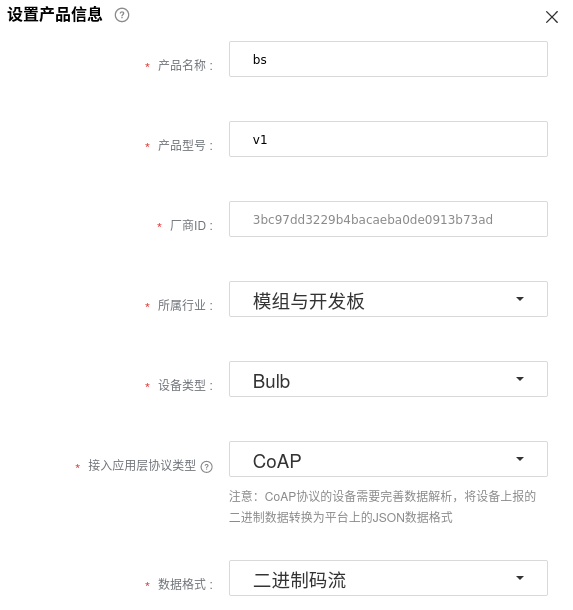
\includegraphics[width=8cm]{oc产品.png}
	\caption{oc产品定义}
	\label{oc产品定义}
\end{figure}


\subsection{定义profile与编解码插件}
profile是描述产品设备信息的文件,定义了设备与应用服务器交互的字段及格式。其主要包含产品信息、服务能力以及维护能力。

实验设备资源主要使用了两个发光二级管以及一个无源蜂鸣器,支持两种操作,分别是触发设备上报设备资源状态和设置设备资源状态,因此设备具有三种属性led0、led1和beep,支持两条下发命令
set\_resource和query\_resource。该设备可用如表\ref{profile格式}的profile文件描述。
\begin{table}[h]
\caption{profile格式}
\begin{tabular}{|c|c|c|c|c|}
\toprule
\multicolumn{5}{|l|}{属性列表} \\
\hline
属性名称 & 类型 & 取值 & \multicolumn{2}{|c|}{描述}  \\
\hline
led0 & int & 0~1 & \multicolumn{2}{|l|}{0:led0关闭 1:led0开启} \\
\hline
led1 & int & 0~1 & \multicolumn{2}{|l|}{0:led1关闭 1:led1开启} \\
\hline
beep & int & 0~1 & \multicolumn{2}{|l|}{0:蜂鸣器关闭 1:蜂鸣器开启} \\
\toprule
\multicolumn{5}{|l|}{命令列表} \\
\hline
命令名称 & 字段属性 & 字段名 & 取值 & 描述 \\
\hline
\multirow{2}{*}{set\_resouce} & 请求 & num & 1-3 & 资源编号 \\
\cmidrule{2-5}
&请求&state&0-1&资源状态 \\
\hline
query\_resouce & 请求 & num & 1-3 & 资源编号 \\
\hline
\bottomrule
\end{tabular}
\label{profile格式}
\end{table}

二进制数据格式需要编解码插件才能解析,在oc平台上设置好profile 文件后,通过将相应属性值与消息模板\ref{消息模板}一一对应,oc平台将会为自身自动生成编解码器,
同时也需要在设备端实现一致的编解码逻辑。


\subsection{接入设备}
华为物联网平台调测可以使用虚拟设备和现实物理设备,当设备侧未开发完成时可以只使用虚拟设备进行调测。对于真实物理设备,华为物联网平台需要设备的唯一标识来认证设备。
此处我选择使用IMEI号。使用PC通过串口连接设备,使用AT+CGSN=1命令查询设备IMEI号,正常情况下设备返回 +CGSN:<IMEI> OK。在oc平台上新增真实设备,填入设备名称和IMEI号,
华为物联网平台将能够识别该设备。
\begin{figure}[h]
	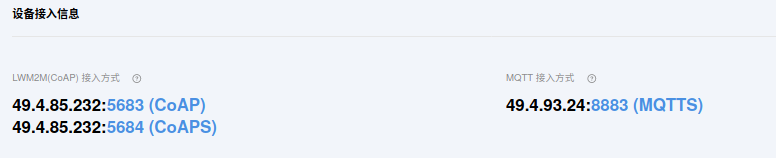
\includegraphics[width=15cm]{oc接入方式.png}
	\caption{oc接入方式}
	\label{oc接入方式}
\end{figure}


\section{stm32终端开发}
stm32终端选择一块搭载stm32f103zet的开发板,板载4组串口,第一组可用于USB通信。本次设计使用到其中第二组串口,对应引脚为PA2和PA3。使用无源蜂鸣器及一组发光二极管,作为设备终端的资源,
对应引脚为PB8,PB5,PE5。使用key0-3,作为外部中断输入,对应模块的初始化、重连和退网,对应引脚为PE2,PE3,PE4。


\subsection{代码设计}
由于通过串口控制BC35G模块运行既是通过发送一系列AT指令,这些指令序列有重复性和相似性,所以将指令视为单元,通过单元的组合完成一个设备功能,比如初始化入网、入网重试、接收消息、发送消息。
以模组关机为例,需要执行关闭网络(\_\_NB\_NETCLOSE)和关闭射频单元(\_\_NB\_CloseCFun)操作,两个操作组合形成功能NBClose,如此能极大方便新功能的增加和旧功能的维护,代码如下:

\begin{lstlisting}
uint8_t (*CloseProc[])()={
        __NB_NETCLOSE,
        __NB_CloseCFun,
};

int8_t __NB_NETCLOSE(){
    char resBuff[UART_BUFFER_SIZE];
    memset(resBuff,0,sizeof resBuff);
    uint8_t res_size;
    char com[30];
    memset(com, 0, sizeof com);
    sprintf(com, NB_CGATT, __NB_ZERO);
    NBCommand((uint8_t*)com, strlen(com), resBuff, &res_size);

    char *strx=NULL;
    strx = strstr((const char *) resBuff, __NB_OK);

    if (strx == NULL) {
        return 0;
    }
    return 1;
}

uint8_t __NB_CloseCFun() {
    char resBuff[UART_BUFFER_SIZE];
    memset(resBuff,0,sizeof resBuff);
    char com[30];
    memset(com, 0, sizeof com);
    sprintf(com, NB_ATCFUN, __NB_ZERO);
    uint8_t res_size;
    NBCommand((uint8_t *)com, strlen(com), resBuff, &res_size);

    char *strx = NULL;
    strx = strstr((const char *) resBuff, NB_OK);

    if (strx == NULL) {
        return 0;
    }
    return 1;
}

uint8_t NBClose(){
    unsigned int it = 0, procNum=sizeof CloseProc;
    procNum=procNum/4;
    for (it = 0; it < procNum; it++) {
        if (!CloseProc[it]()) {
            NBERROR(it);
            it--;
        }
    }
    return 1;
}
\end{lstlisting}

\subsection{串口DMA通信}

stm32开发板控制bc35g模块是通过串口的方式,bc35g串口比特率为9600。为了接收变长的串口数据,可以有以下几种方式:

BC35G模块串口传输数据以'lr cr'为分隔符,以软件的方式,设置超时接收固定长度并以'lr cr'分割,放入缓冲区中。由于模块涉及网络操作等原因,不同AT指令的响应时间有很大差距,所以超时时
间不好确定,同时由于MCU等待模块输入,对效率影响较大。

利用定时器中断方式可以解决超时时间设置的问题。一个字节的数据有 起始位+数据+结束位共10位,在模块串口比特率为9600的情况下,传输一个字节需要104us。同时由于两组数据之间需要间隔3.5字
符,可以设置定时器中断为5ms。在串口接收中断服务函数中开启定时器中断,每接收一个字符则重置定时器,当定时器超时时可以认为一组数据接收完毕,在定时器中断函数中将接收到的数据放入缓存中。
但是由于是一字节一字节接收,而且MCU仍然参与接收过程,所以效率仍有提升必要。

为了进一步提升效率,可以使用DMA方式接收数据。为了区分两组数据,开启总线空闲中断,当DMA传输完毕时触发总线空闲中断,在总线空闲中断中标记数据就绪。DMA方式能获得更好的效率。

\begin{lstlisting}
/* uart.c
* 检测空闲中断,标记缓存数据可用
*/

uint8_t UART2DATAREADY = 0;
uint8_t UART2RXBUFFER[UART_BUFFER_SIZE];

void USER_UART_IRQHandler(UART_HandleTypeDef *huart) {
    if (huart == &huart2) {
        if (RESET != __HAL_UART_GET_FLAG(&huart2, 
                UART_FLAG_IDLE)) {
            __HAL_UART_CLEAR_IDLEFLAG(&huart2);
            HAL_UART_DMAStop(&huart2);
            UART2DATAREADY = UART_BUFFER_SIZE - 
            __HAL_DMA_GET_COUNTER(&hdma_usart2_rx);
        }
    }
}

/* nbiot.c
* 封装AT指令执行模块,接收模块串口回传数据
*/
func NBCommand(AT_command) {
    UART_Transmit(AT_command);
    HAL_UART_Receive_DMA(&huart2, 
                        UART2RXBUFFER, 
                        UART_BUFFER_SIZE);
    Delay(100); //降低UART2DATAREADY datarace概率
\end{lstlisting}    

\subsection{初始化及入网}
BC35G模块初始化需要首先使用AT+NCDP=<ip,port>命令设置云平台CoAP协议接入地址,该地址可以从华为物联网平台的项目对接信息中获取。

根据USIM卡对应的不同运营商和表\ref{运营商band分配},使用AT+NBAND=<band>命令设置设备运行频段。

同时为了达到固定控制类应用对时延的要求,需要使用AT+CEDRXS=0,5和AT+CPMS=0关闭edrx和省电模式PSM。

模块默认开启数据自动上报,当接收到物联网平台消息是就会自动通过串口上报。由于为了避免与stm32的控制消息在串口结合在一起后期分离不变,所以使用AT+NNMI关闭串口数据自动上
报,定时按需使用AT+NQMGR和AT+NMGR从缓存中获取消息。
最终触发入网并查询入网状态,需要执行的流程及AT指令如图\ref{入网流程}

\begin{figure}[H]
    \centering
	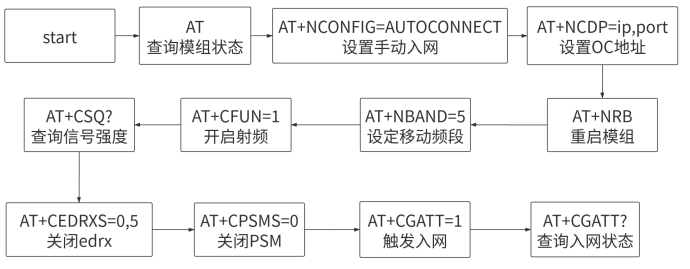
\includegraphics[width=13cm]{入网流程.png}
	\caption{入网流程}
	\label{入网流程}
\end{figure}


如果入网失败,可以尝试重连,重练操作序列如图\ref{入网重试}

\begin{figure}[H]
    \centering
	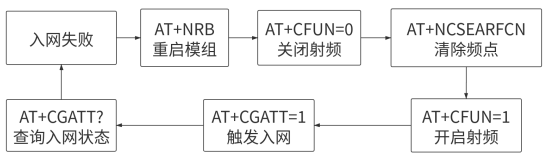
\includegraphics[width=13cm]{入网重试.png}
	\caption{入网重试}
	\label{入网重试}
\end{figure}

当设备不处于第一次开机的流程,入网操作只需要打开射频功能以及触发入网,如图

\subsection{模组通信}

bc35g模块涉及消息发送与接收的有如下四个命令:
\begin{table}[h]
\caption{bc35g模块收发命令}
\begin{tabular}{|c|c|}
\toprule
命令 & 描述 \\
AT+NMGS=<length>,<data> & \makecell[l]{data为16进制数据,length为data长度,\\用于向IOT平台发送数据} \\
AT+NIMI=0/1 & \makecell[l]{关闭/开启自动上报,模块接收到消息是会\\自动发往串口} \\
AT+NQMGR & \makecell[l]{查询自开机以来接收到的消息状态} \\
AT+NMGR & \makecell[l]{读取缓存中最早一条未被未被处理的消息} \\
\bottomrule
\end{tabular}
\label{tablea}
\end{table}

如果开启自动上报,则服务器下发内容有可能与串口控制消息重叠,需要消耗额外资源去提取。同时由于固定控制类应用对延时要求较高,所以关闭自动上报,定时轮询缓存中是否有接收到新消息。

\begin{lstlisting}

//nbiot.c
func readMsg(){
    received=NBCommand("AT+NQMGR")
    for read to received{
        data+=NBCommand("AT+NMGR")
    }
    data+="command_end"
    read=received;
    return data;
}

//main.c
while(1){
    Delay(1000);
    data=readMsg();
    process(data);
}
\end{lstlisting}


\subsection{退网关机}

当设备关机时需要释放与运营商的连接,须执行以下序列\ref{模块关机}
\begin{figure}[H]
    \centering
	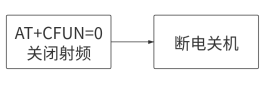
\includegraphics[width=7cm]{模块关机.png}
	\caption{模块关机}
	\label{模块关机}
\end{figure}

\section{验证过程以及结论}

首先使用PC串口通信的方式,控制模块通信操作,使用的AT指令以及结果如图\ref{PC命令行实验}:


\begin{figure}[H]
    \centering
	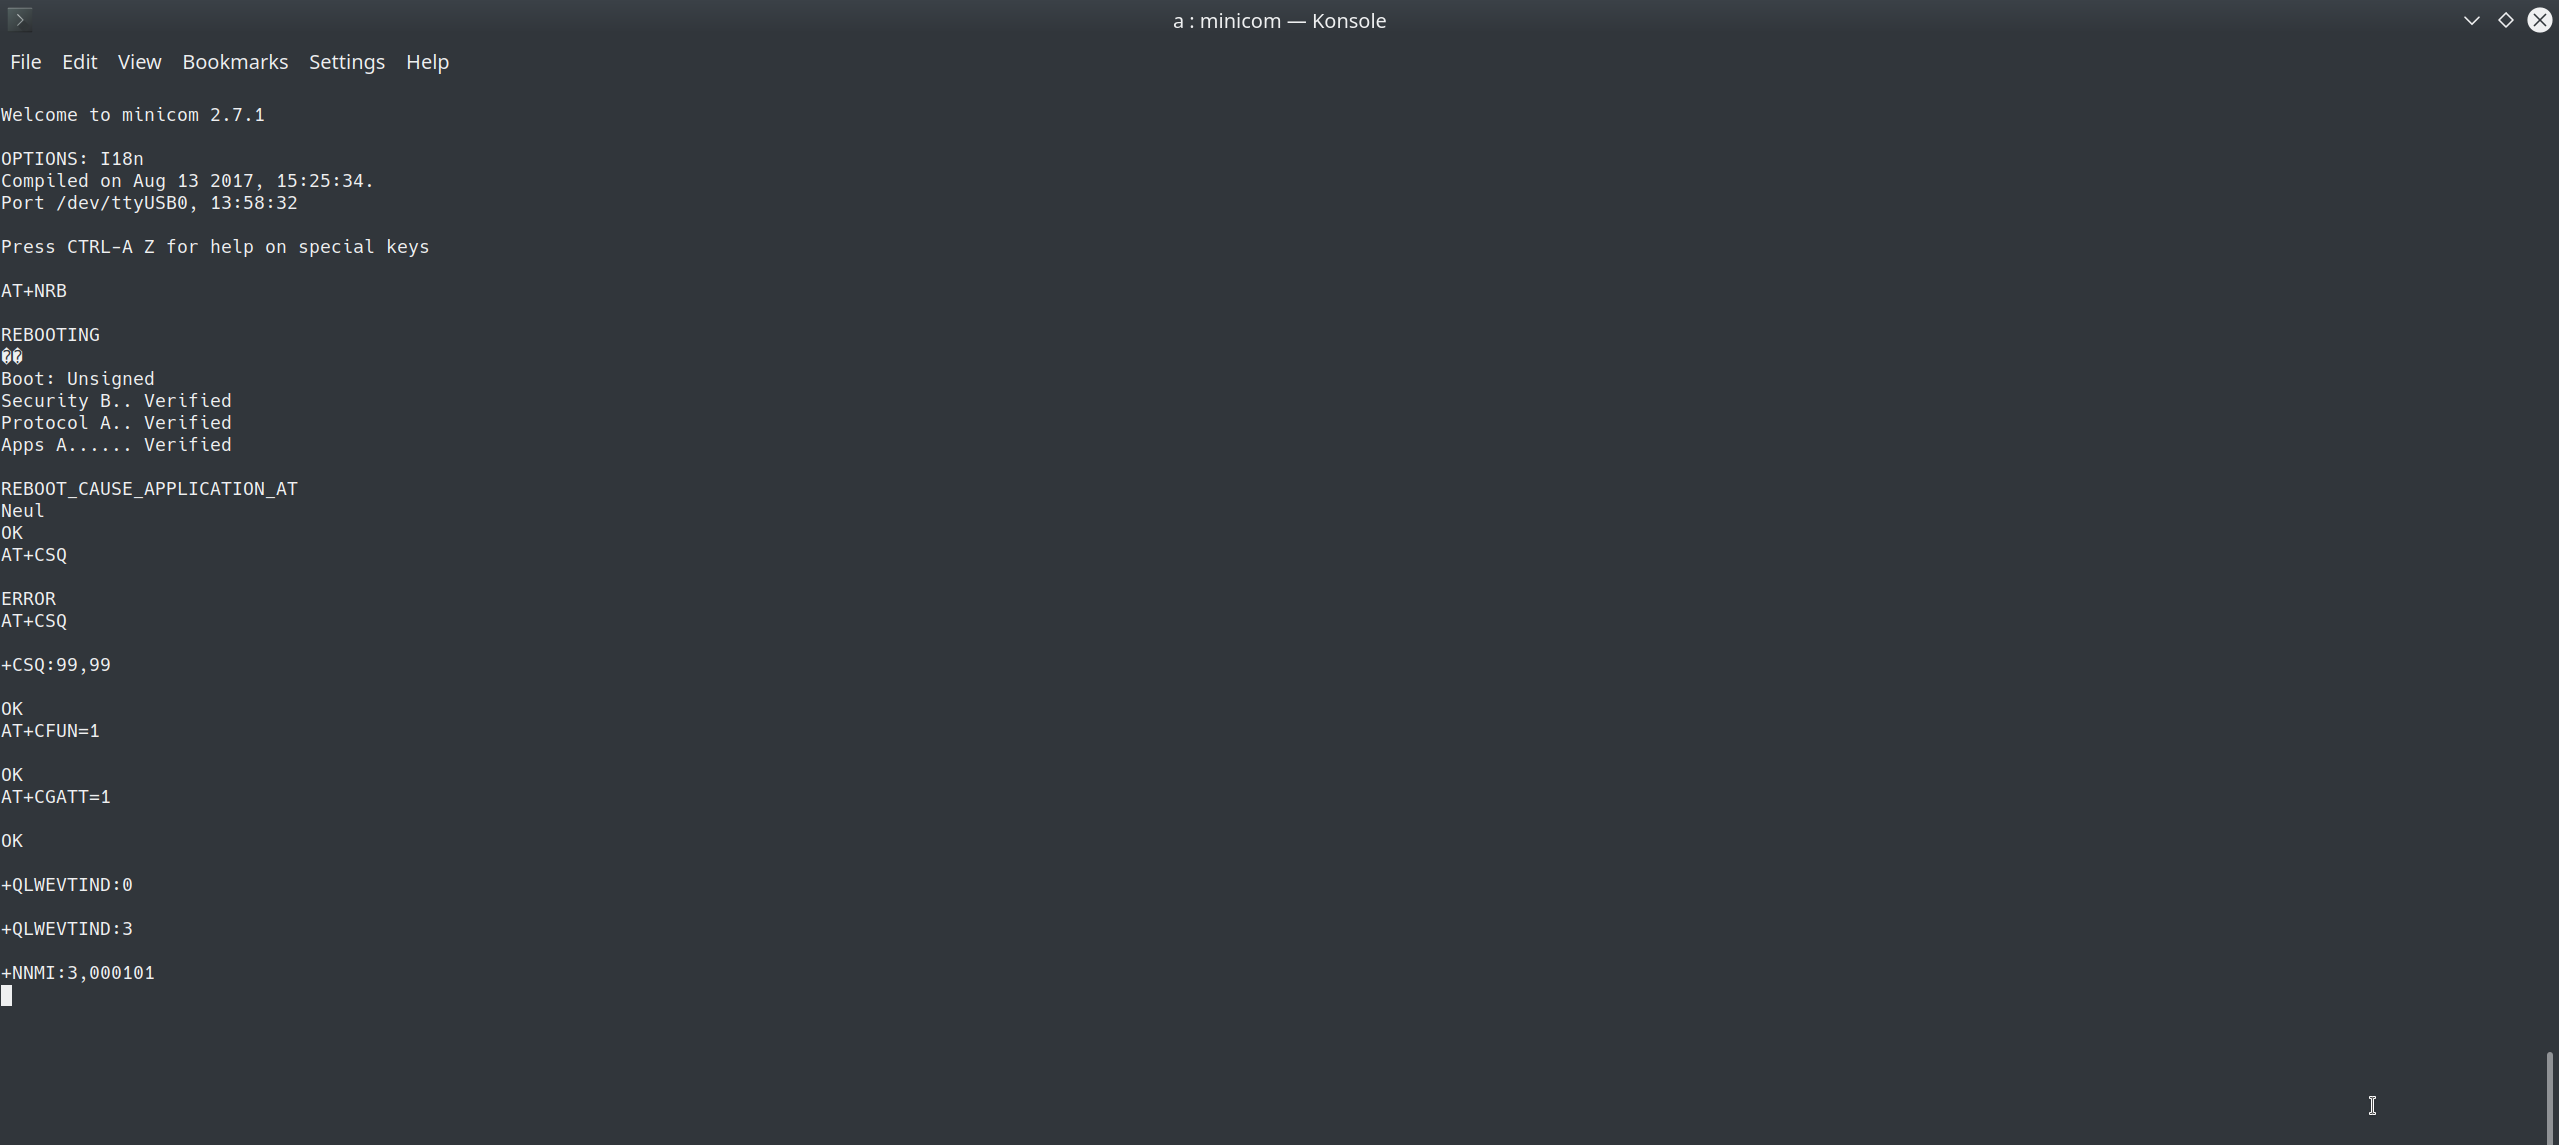
\includegraphics[width=10cm]{PC命令行实验.png}
	\caption{PC命令行实验}
	\label{PC命令行实验}
\end{figure}

设备未入网时LED全灭,华为OC平台显示设备离线,两者状态如图\ref{设备离线端}、图\ref{设备离线}

\begin{figure}[H]
    \centering
	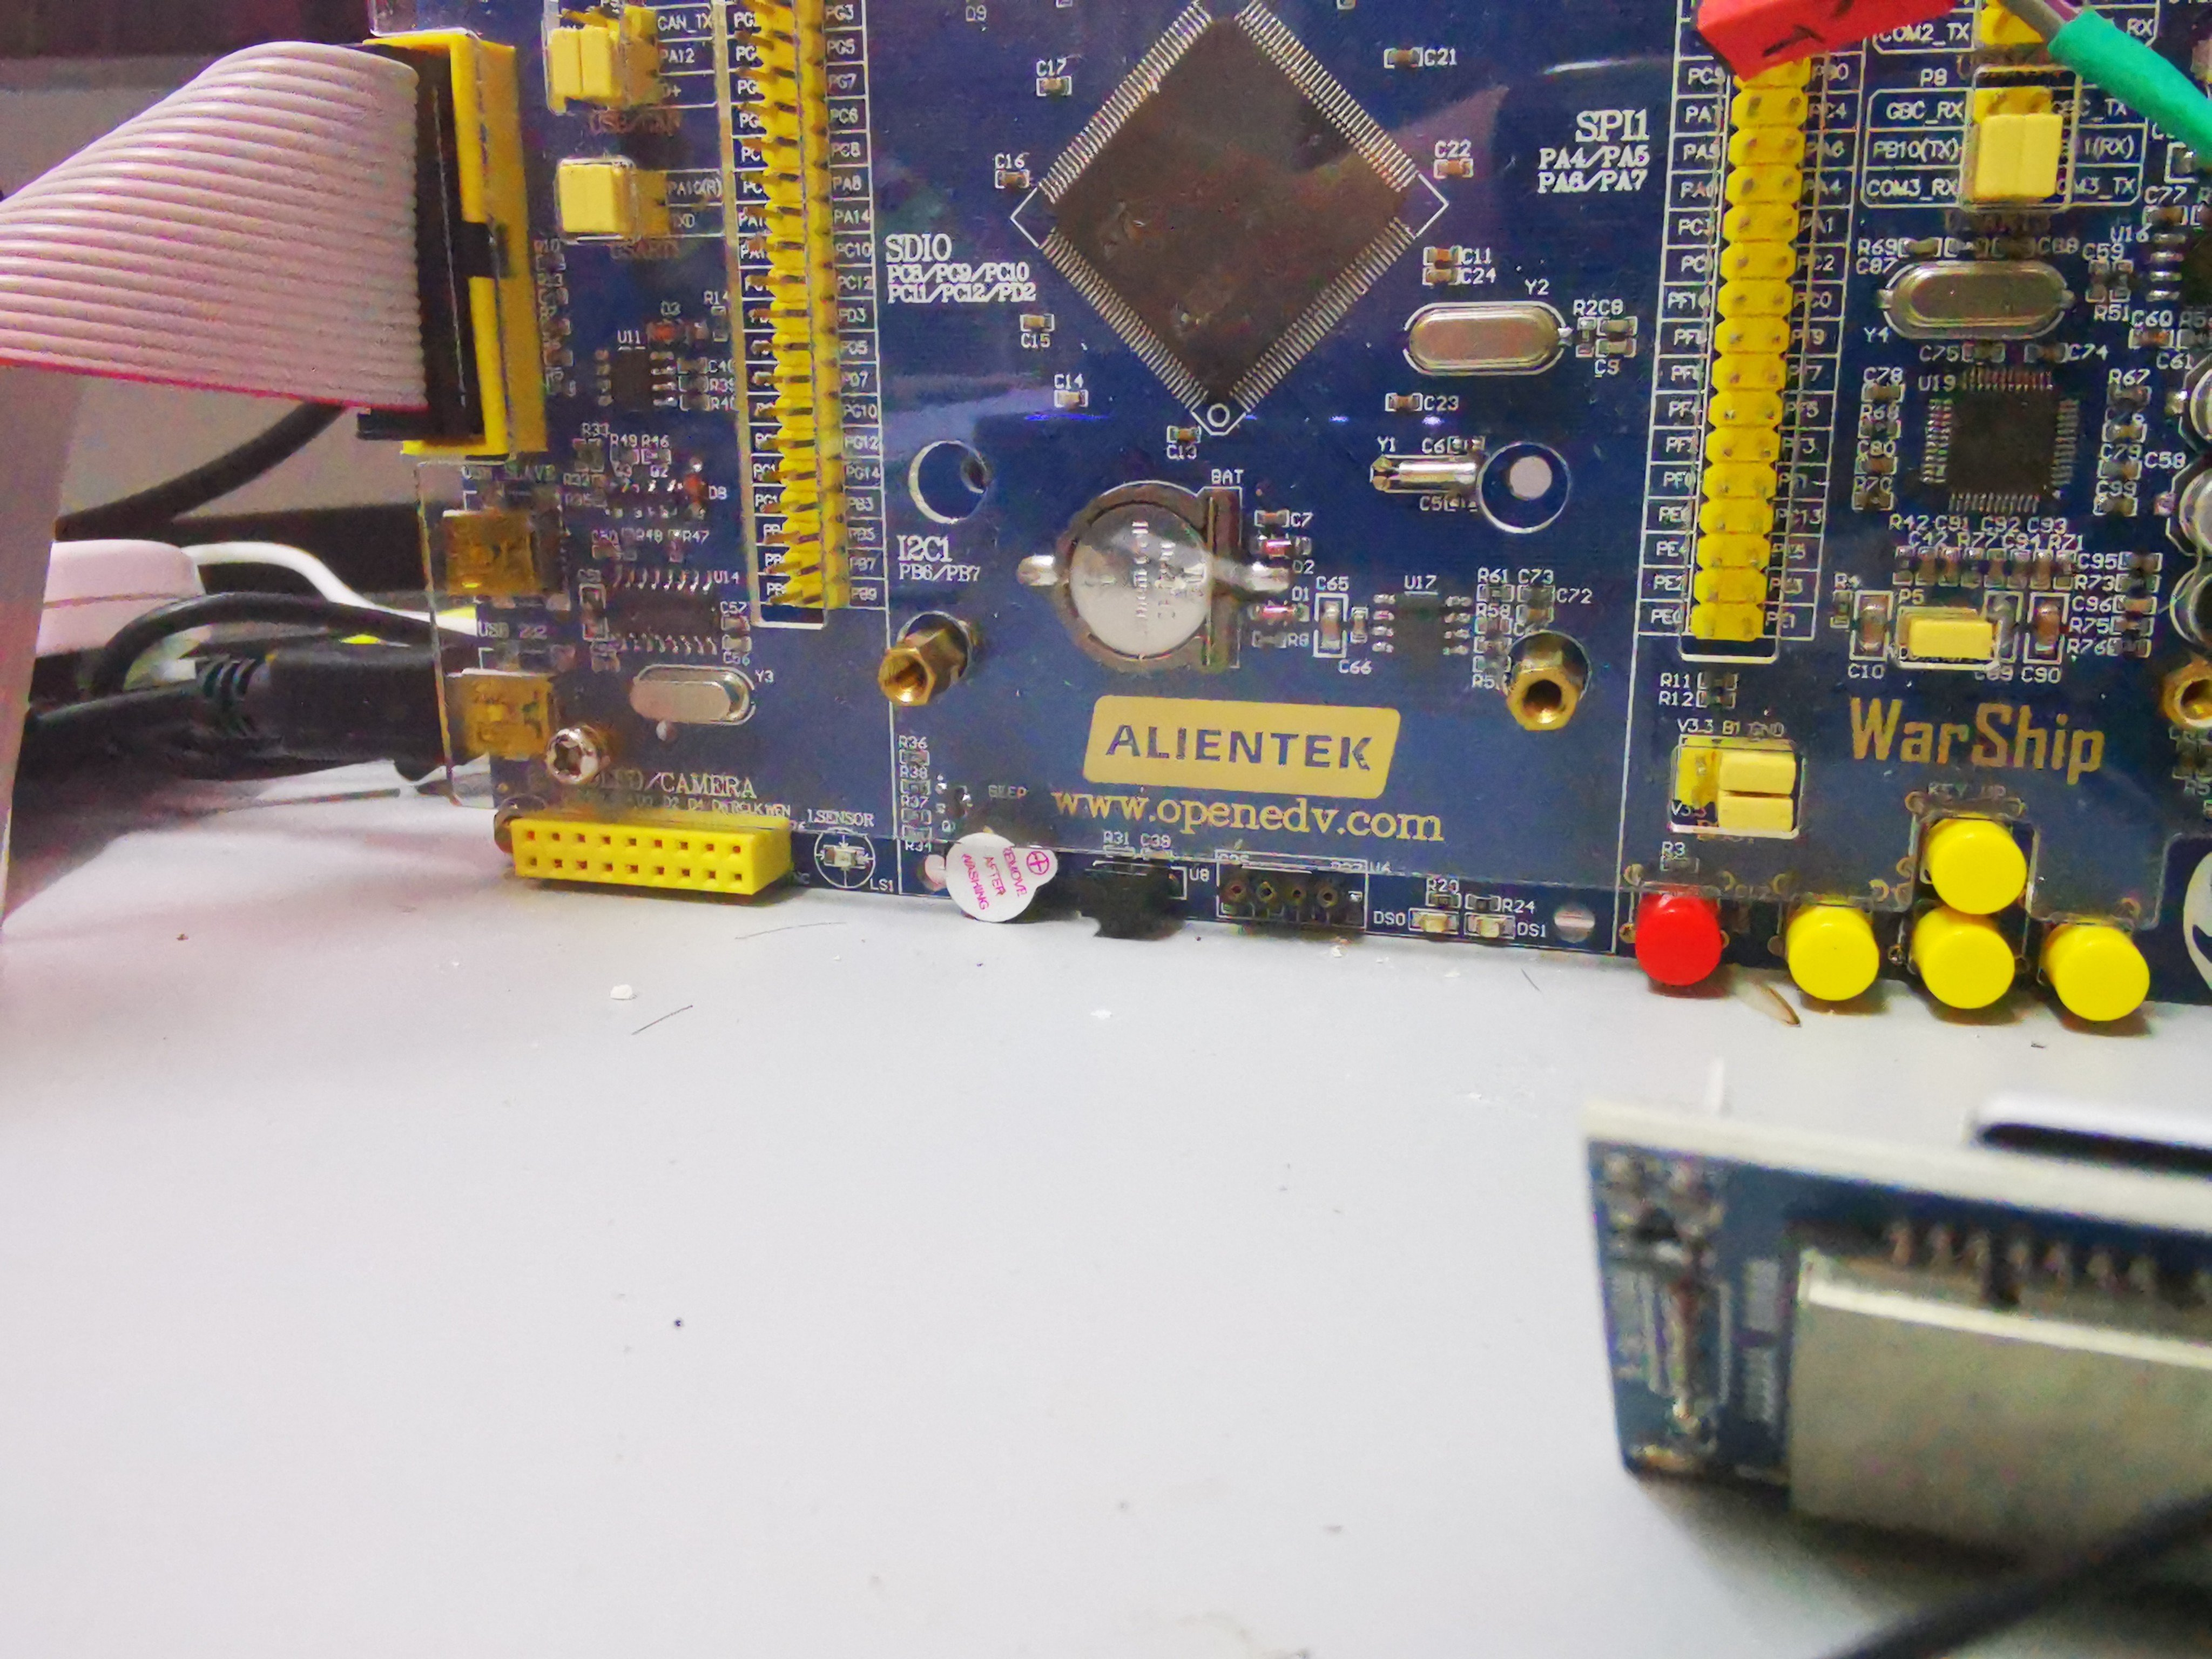
\includegraphics[width=7cm]{设备离线端.png}
	\caption{设备离线端}
	\label{设备离线端}
\end{figure}


\begin{figure}[H]
    \centering
	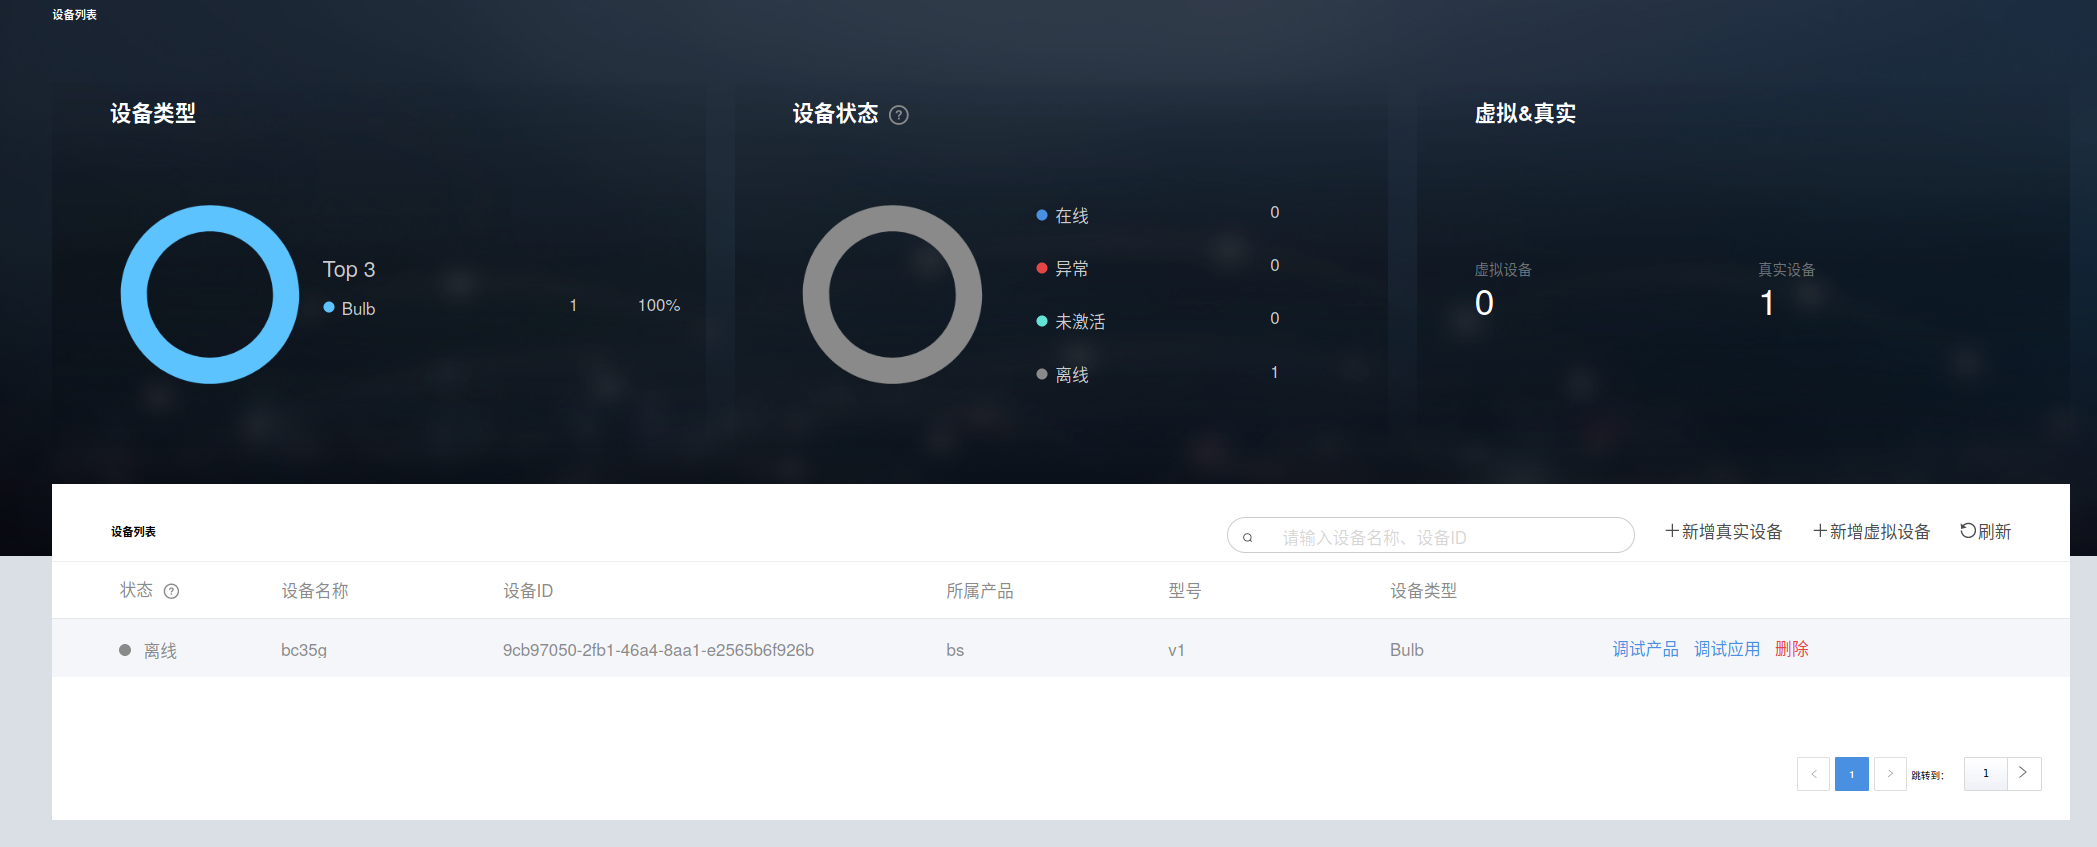
\includegraphics[width=7cm]{设备离线.png}
	\caption{设备离线}
	\label{设备离线}
\end{figure}

入网成功后,红色LED0亮起,华为OC平台显示设备上线
\begin{figure}[H]
    \centering
	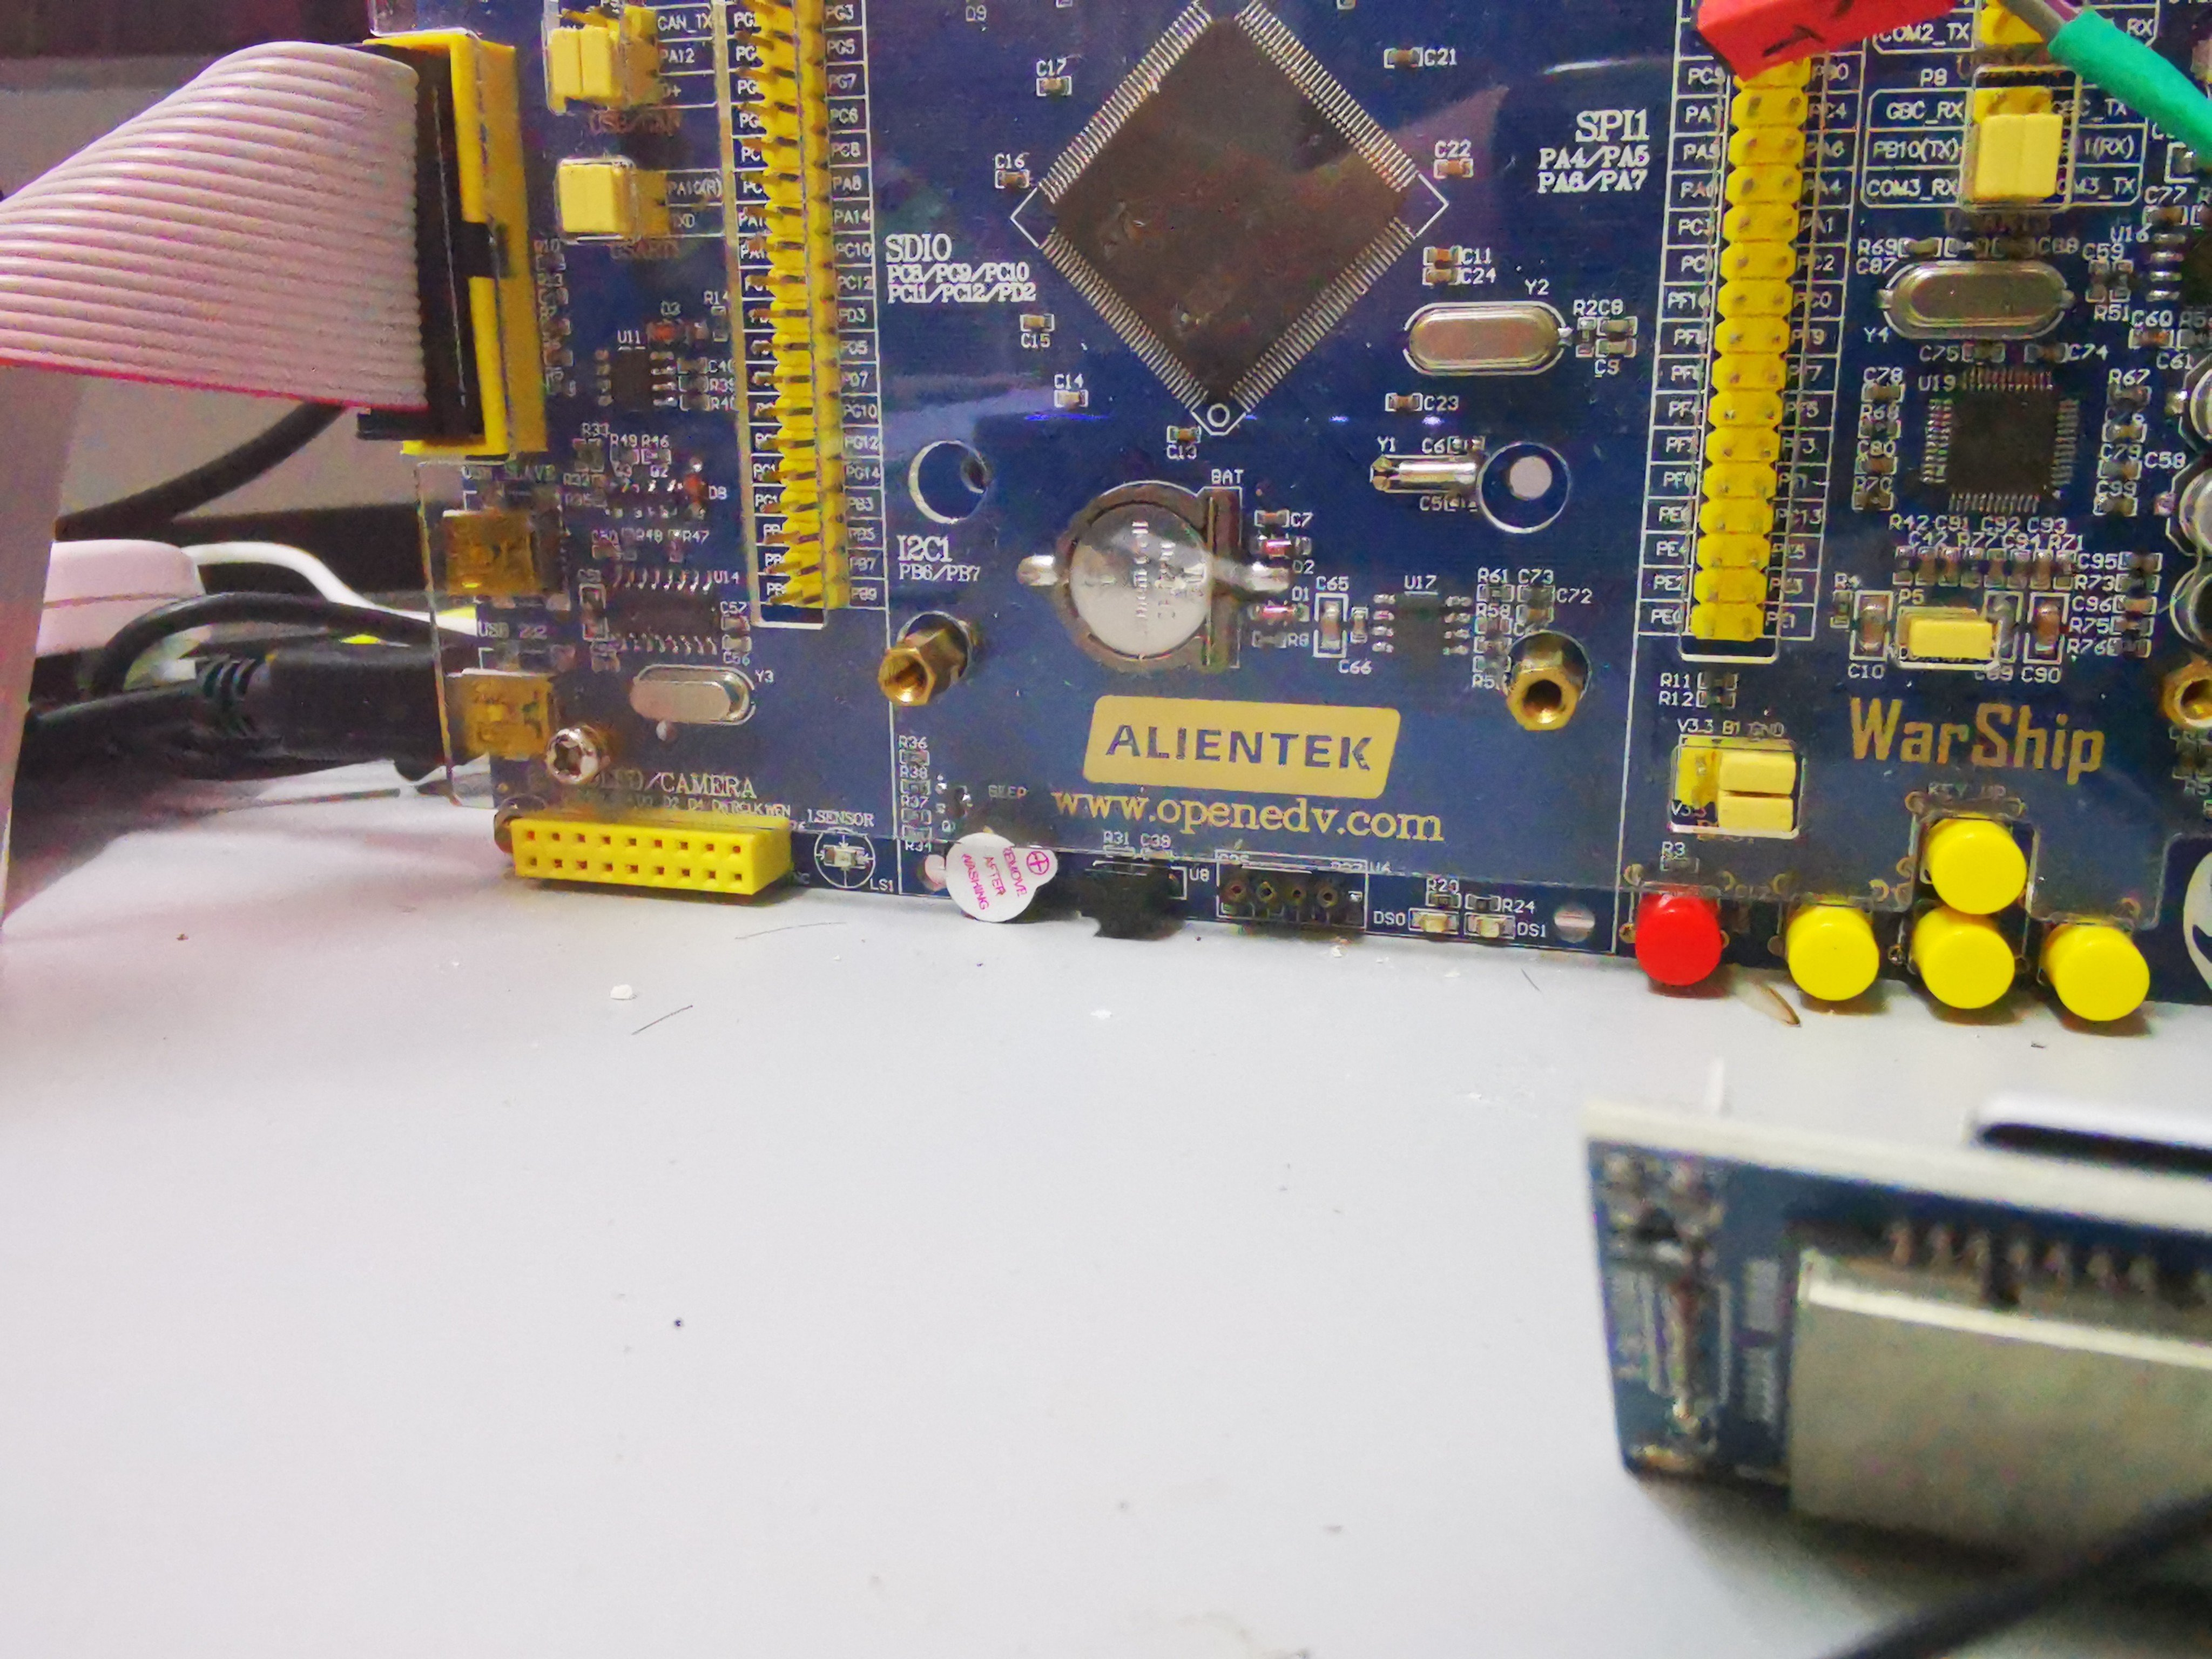
\includegraphics[width=7cm]{设备离线端.png}
	\caption{设备上线端}
	\label{设备上线端}
\end{figure}


\begin{figure}[H]
    \centering
	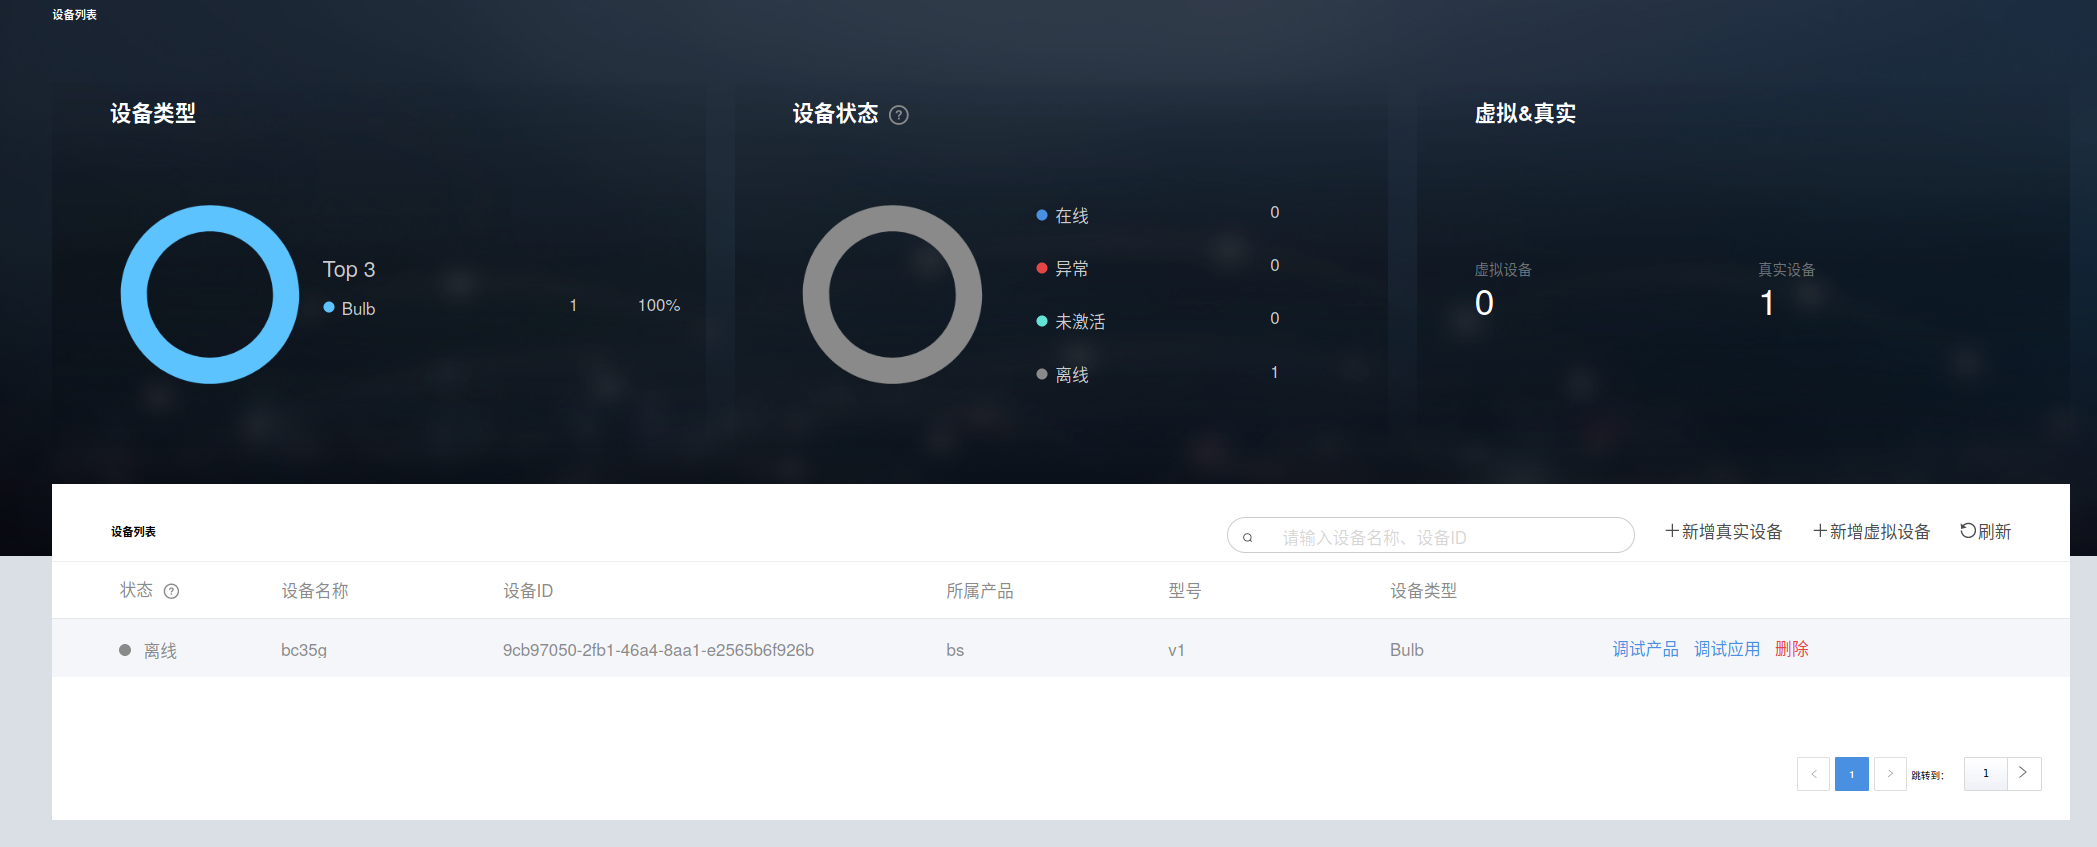
\includegraphics[width=7cm]{设备离线.png}
	\caption{设备上线}
	\label{设备上线}
\end{figure}

通过下发控制命令开启、关闭LED灯和触发设备信息上报,设备端和云端状态如下:
\begin{figure}[H]
    \centering
	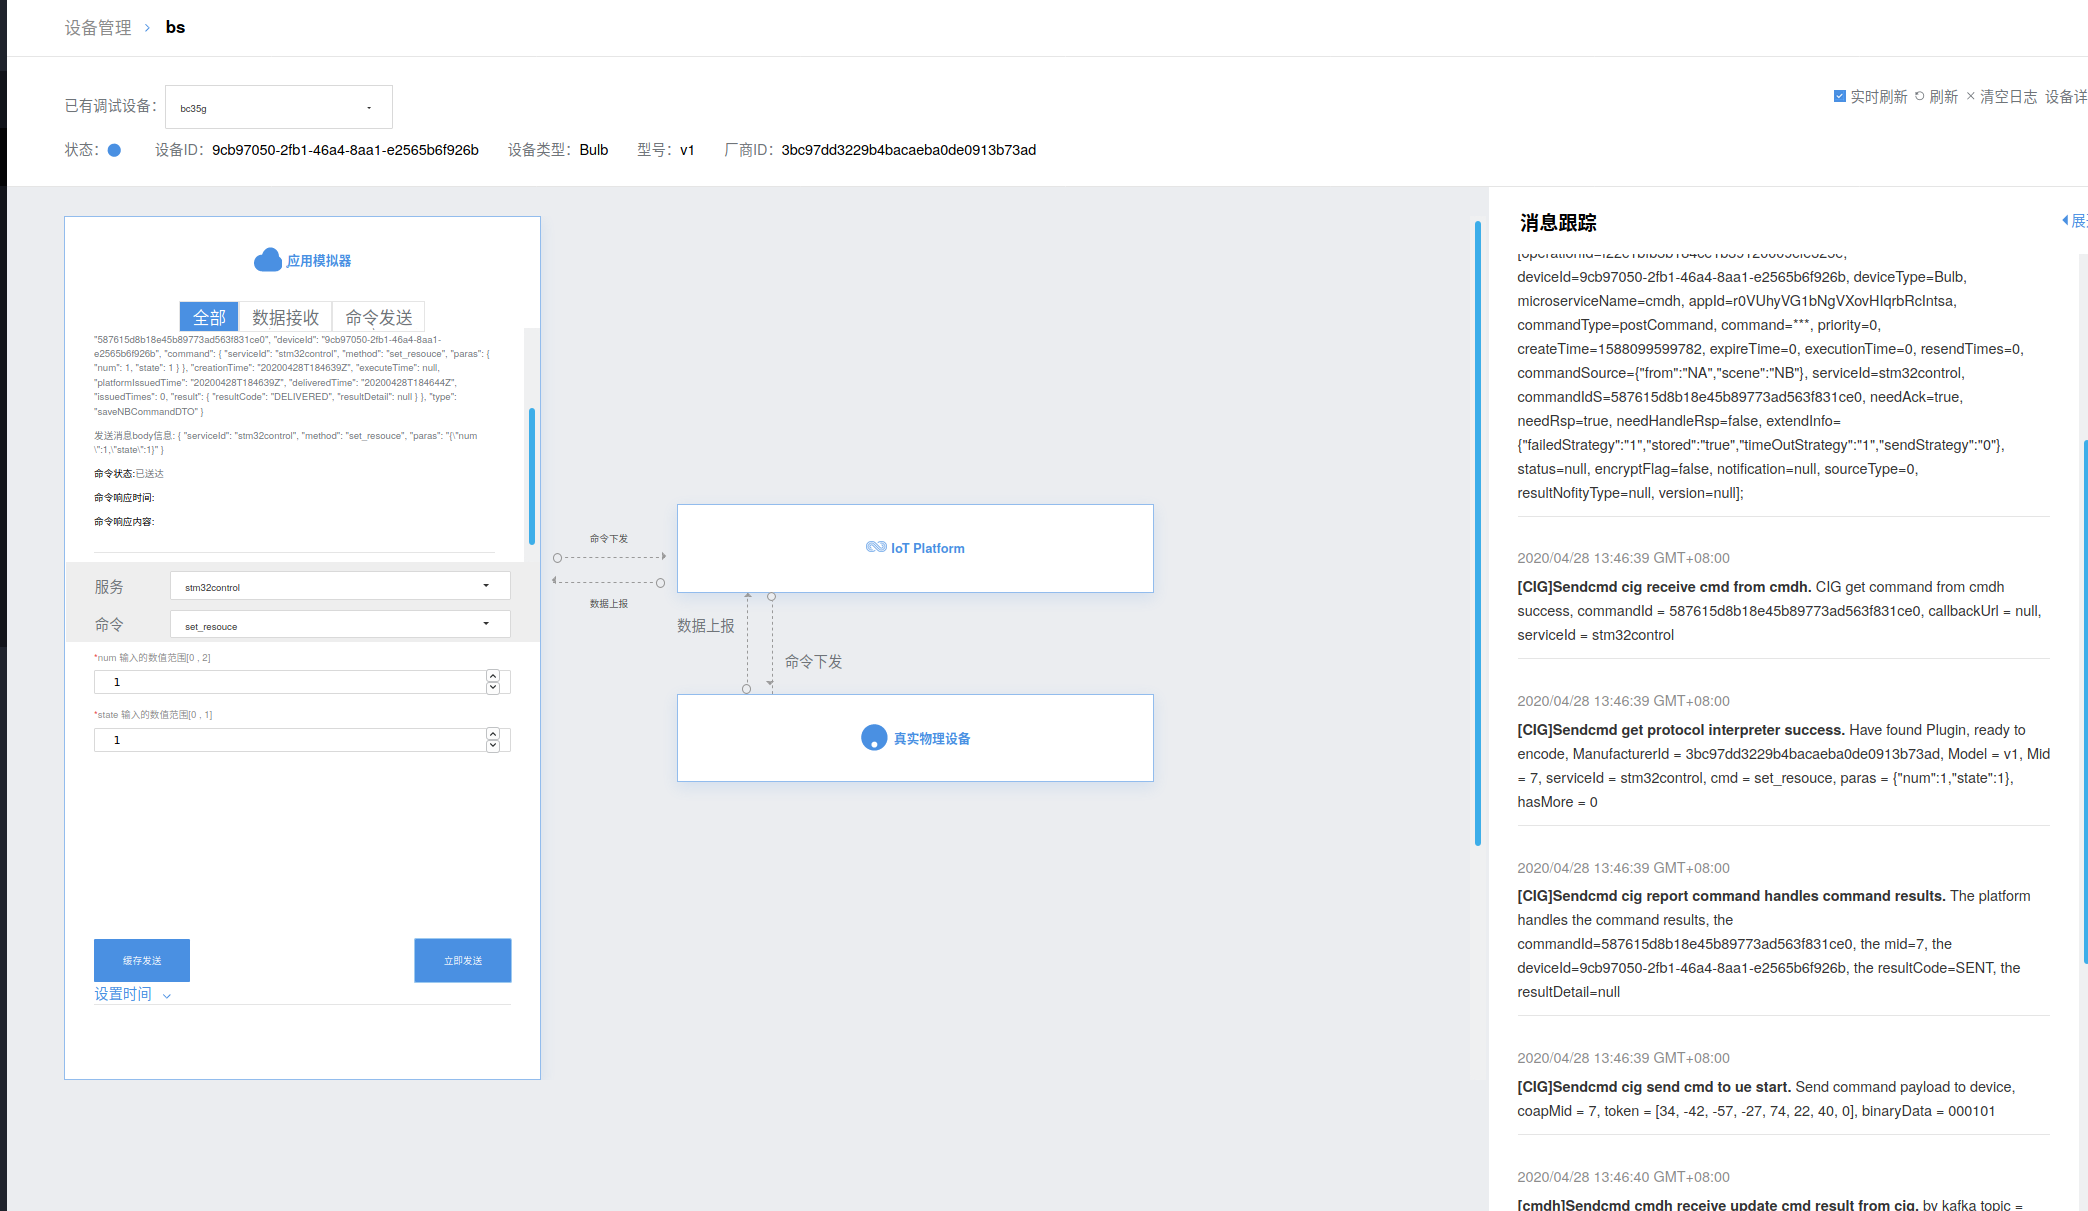
\includegraphics[width=7cm]{发送开灯.png}
	\caption{发送开灯}
	\label{发送开灯}
\end{figure}


\begin{figure}[H]
    \centering
	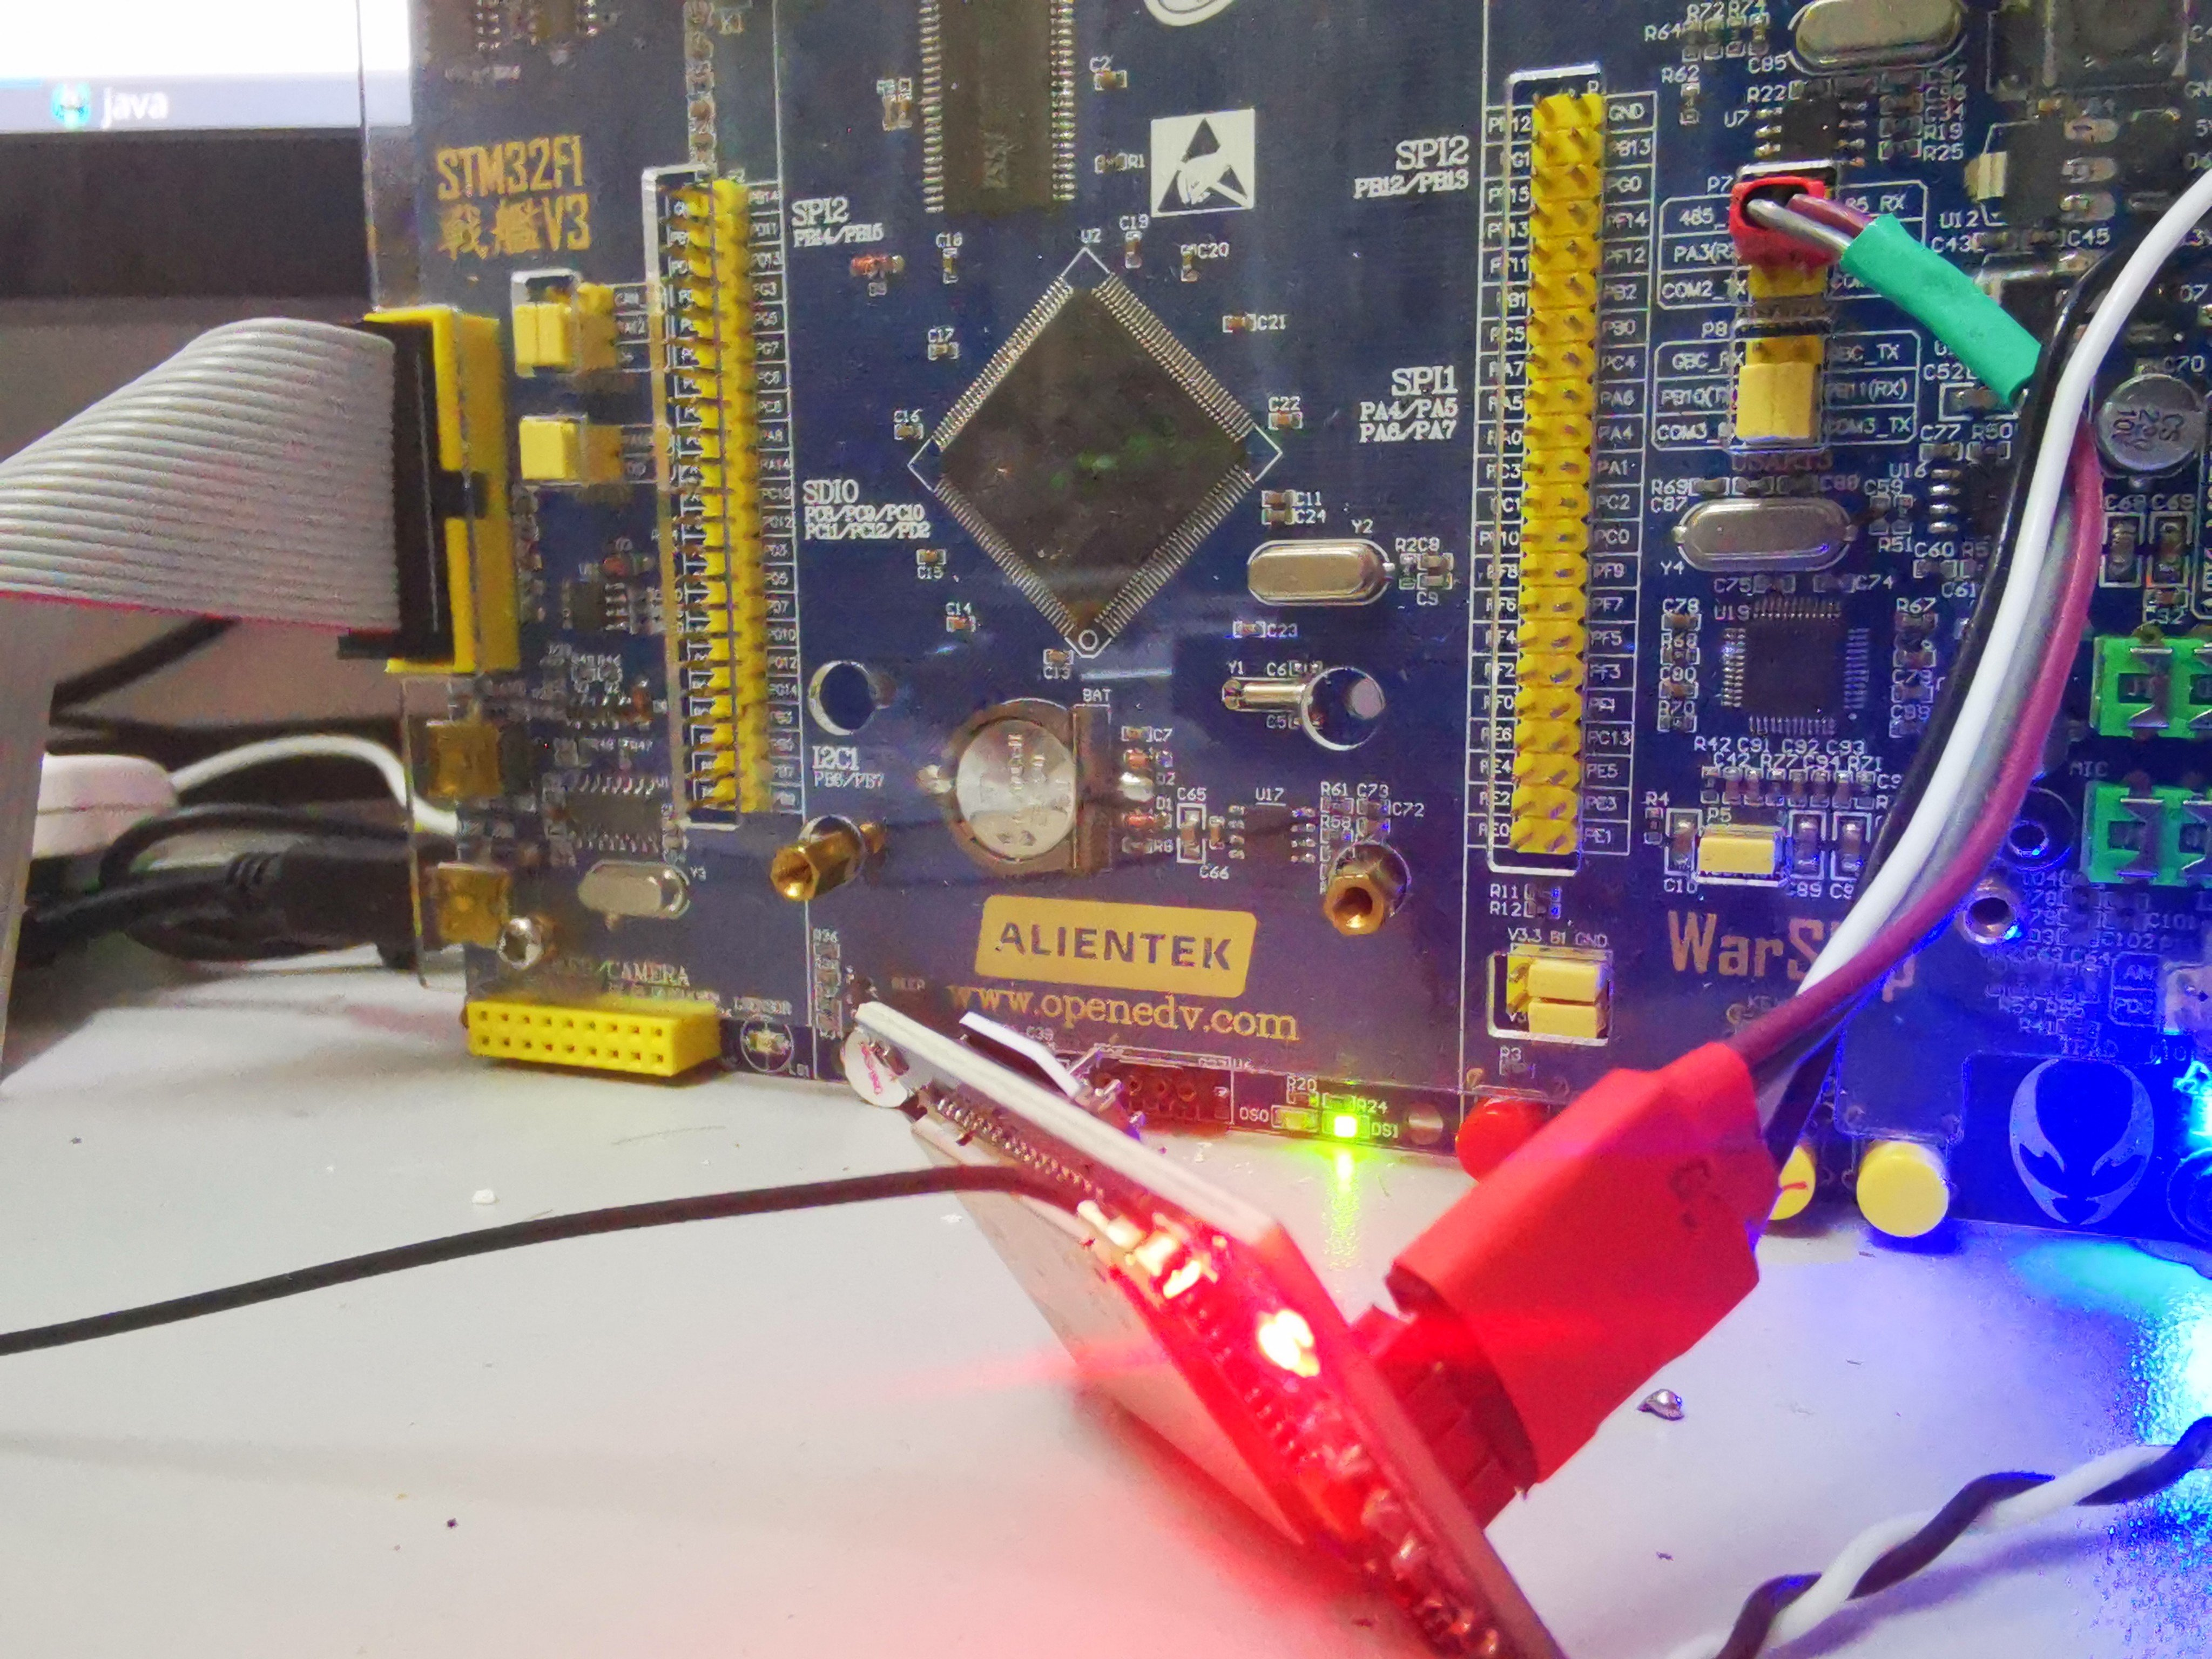
\includegraphics[width=7cm]{发送开灯端.png}
	\caption{发送开灯端}
	\label{发送开灯端}

\end{figure}\begin{figure}[H]
    \centering
	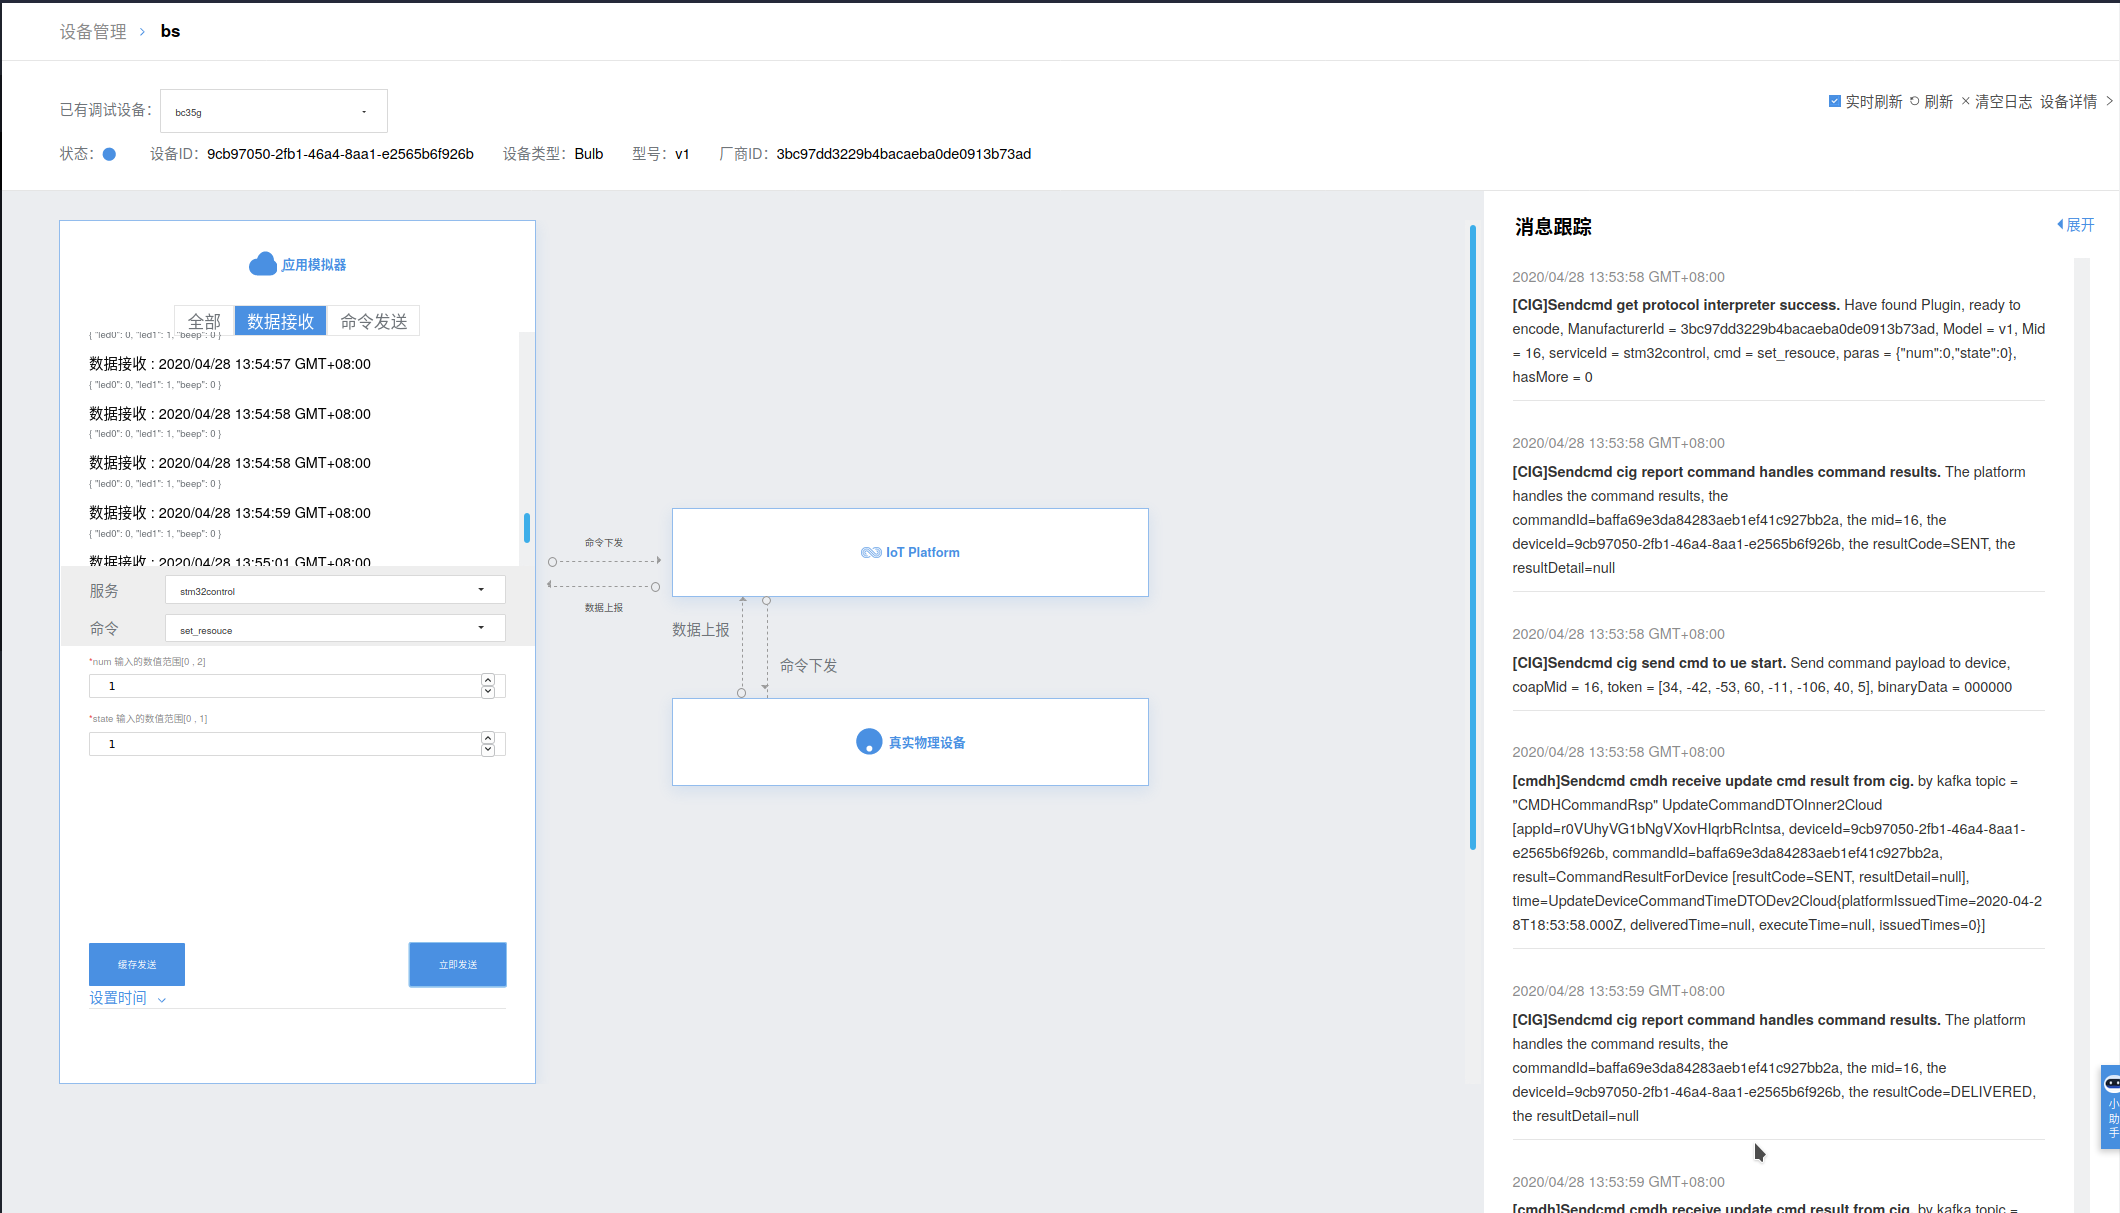
\includegraphics[width=7cm]{设备上报.png}
	\caption{设备上报}
	\label{设备上报}
\end{figure}

\section{本章小结}

本章通过简单模拟一个固定控制类应用,在STM32开发板上实现对BC35G模块的通信控制,通过CoAP协议,完成查询、上报、控制资源状态三种消息类型的传输,验证了BC35G模块的功能